\documentclass{ctexart}
%\CTEXsetup[name={Step ,},number={\arabic{chapter}}]{chapter}

\usepackage{amsmath}
%\usepackage{wallpaper}
\usepackage{xcolor}
%\usepackage{pgf, tikz}
\usepackage{multirow}
\usepackage{listings}
\usepackage{color}

\definecolor{keywordcolor}{rgb}{0.8,0.1,0.5}
\definecolor{webgreen}{rgb}{0,.5,0}

%\usepackage[paperwidth=185mm,paperheight=260mm,text={148mm,210mm},left=21mm,includehead,vmarginratio=1:1]{geometry}
%\usepackage[raggedright]{titlesec}
%\titleformat{\chapter}[display]{\Huge\bfseries}{Step \,\thechapter\,}{1em}{}

%\usepackage{fancyhdr}
%\pagestyle{fancy}
%\fancyhf{}
%\fancyhead[ER, OR]{\leftmark}
%\fancyhead[EL, OL]{《编译实习》实习报告}
%\fancyfoot[C]{\thepage}
%\renewcommand{\chaptermark}[1]{\markboth{\thechapter.\ #1}{}}


\lstset{language=C,
basicstyle=\footnotesize,
keywordstyle=\color{keywordcolor}\bfseries, %\underbar,
identifierstyle=,
commentstyle=\color{green} \textit,
stringstyle=\color{red} \ttfamily,
showstringspaces=false,
frame=single,
numbers=left,
numberstyle=\tiny \color{blue},
backgroundcolor=\color{white},
captionpos=b
}


\begin{document}

\title{%
\vspace{-30mm}\heiti\Huge NachOS Lab1 实习报告 \vspace{10mm}}
\author{%
\Large 史杨勍惟 
\\[10mm] 1200012741 信息科学技术学院}
\date{2016,03,15}

\maketitle

\newpage
\tableofcontents
\newpage

\section{总体概述}
这次Lab主要是对Nachos线程机制的理解和扩充。
其中扩充的部分内容比较少,主要作用是还是在于加深线程机制的理解。以及对不同操作系统的线程机制的理解。

虽然这次的工作量比较小,但是我还是看到了设计一个底层的系统所需要的系统性和复杂性。所谓系统性就是在设计的时候需要从整个系统进行考虑,而不是针对单一功能。所谓复杂性就是要考虑地比较细节,以保证系统的正常运行。

总的来说,这次的主要任务在于对线程机制的理解,在此基础上,做了简要的扩充,添加维护了一些成员,增加了限制,以及实现了一个简单的输出功能。

\section{任务完成列表}
\begin{table}[h]
\centering
\footnotesize
\begin{tabular}{|c|c|c|c|}\hline
\textbf{Exercise 1} & \textbf{Exercise 2} & \textbf{Exercise 3} & \textbf{Exercise 4} \\\hline
Y & Y & Y & Y \\\hline

\end{tabular}

\end{table}
\section{完成情况}
\subsection*{Exercise 1}
\textbf{调研Linux或Windows中进程控制块的基本实现方式,理解与Nachos的异同}

首先,我们来看一下Linux中的进程管理比较复杂:
Linux为每个线程维护了一个threadinfo,在threadinfo中有一个很重要的数据结构叫taskstruct,这就是Linux中的进程控制块。Linux进程控制块中有很多属性,如状态,权限,id,父进程等等。Linux不区分进程线程,只不过进程线程的属性会有不同。taskstruct有一个slab分配器进行统一分配,能够达到对象复用和缓存着色等目的。

相比之下,Nachos和Linux一个比较相似的地方在于Nachos也不分进程和线程,都以线程为单位。但是Nachos中的线程结构比Linux中的要简单很多很多,只有一些基本的线程属性。而且分配过程也非常简单,直接调用C++的new即可。
\subsection*{Exercise 2}
\textbf{阅读源代码,理解Nachos现有的线程机制}
thread.cc和thread.h是核心,主要有四个主要接口分别是
\begin{enumerate}
\item Fork: 线程的创建,通过底层的栈分配使得线程的第一条命令指向一个用户的函数。
\item Finish: 线程的结束。
\item Yield: 线程执行和切换的触发。
\item Sleep: 线程的挂起。切换到其他线程。
\end{enumerate}

每次Fork出来的线程都是被放到最后的,所以说我们可以推断出Nachos现在的调度方法是``先到先得''。

threadtest是一个对thread的测试,从中我们可以看到时序相关的信息。其实在创建线程后线程并不会运行,只有Yield了的时候才会真正触发线程运行。在这个threadtest中,两个线程轮换地相互Yield所以就造成了最后轮换运行的输出结果。

\subsection*{Exercise 3}
\textbf{增加用户ID,线程ID两个数据成员}
数据成员的增加非常简单,只需要如下在Thread数据结构中增加相应的成员即可
\begin{lstlisting}
private:
  int uid;
  int tid;
\end{lstlisting}

\textbf{在Nachos现有的线程管理机制中增加对这两个数据成员的维护机制}

主要维护的工作在于初始化的时候两个ID的分配。

UID是用户的ID,应该由用户来确定。在现有的Nachos代码中还没有用户区分的功能。再次我使用了C++的函数默认参数功能让用户在创建线程的时候可选地设置UID。

TID的分配室友线程分配器分配的。对于分配器的实现方式主要有两种,一种是基于位图的,一种是基于链表的。在此我采用了后者,因为这样再分配的时候只需要O(1)的时间就可以了。我是用的工具是C++ STL中的list。其实我后来发现Nachos中本身就有List工具,可以现用。不过发现的时候我已经写完这个部分了,所以也没有使用现有的List。

我的分配函数如下:
\begin{lstlisting}
int allocateTID() {
    if(threadAllocator.empty()) {
        return -1;
    } else {
        int ret = threadAllocator.front();
        threadAllocator.pop_front();
        return ret;
    }
}
\end{lstlisting}

此函数被添加到了Thread的构造函数中。

与分配函数对应的是释放函数,这个比较简单,只要把TID重新加回链表即可。所以我只是简单的把语句添加到了析构函数中,没有单独写函数了。

另外我也在Thread结构中添加了这两个成员的getter函数,getUID和getTID,我把这个集成到最后的TS功能上了,所以在此就不展示了。

\subsection*{Exercise 4}
\textbf{在Nachos中增加对线程数量的限制,是的Nachos中最多能够同时存在128个线程}

正如上面这个练习中所设计的,空闲线程被出示化成列表,所以只需将这个链表初始化成128个元素就行了,这个只需要修改宏定义即可。这个练习主要的难点在于线程超出限额的处理方式。我认为主要可以采取下面三种方式。
\begin{enumerate}
\item 直接退出系统。
\item 不创建该线程。
\item 睡眠直到有空闲链表有余。
\end{enumerate}

第一种方式相对来说最方便,但是这种方式会产生内存泄漏的问题。第三种方式比较复杂,需要涉及线程间通信的相关问题。所以中和来看,我选择了第二种方法。由于创建线程的本质是调用了Fork接口,所以只要在Fork成员函数中添加一个判断就行,如果空闲链表没有多余,直接返回即可。

在这里我设计了如下的测试
\begin{lstlisting}
void doVoid(int tid) {
    printf("forked thread run with tid %d\n", tid);
    return;
}

void ThreadTest2() {
    DEBUG('t', "Entering ThreadTest2");
    for(int i = 0; i <= 129; ++i) {
        Thread *t = new Thread("forked thread");
        t->Fork(doVoid, t->getTID());
    }
}
\end{lstlisting}

得到的结果是
\begin{figure}[h]
 \centering
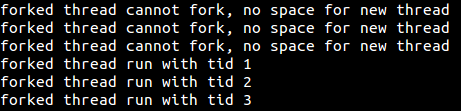
\includegraphics[width=4in]{ex2.png}
\end{figure}

由于没有主动触发运行,所以所有的fork线程都是在退出的时候被触发的,所以在创建第128个线程的时候会有报错,因为已经有127个还在等待的线程以及main线程了。

为了探究时序的问题,我对ThreadTest2做了小小的修改,添加了一句Yield

\begin{lstlisting}
void ThreadTest2() {
    DEBUG('t', "Entering ThreadTest2");
    for(int i = 0; i <= 129; ++i) {
        Thread *t = new Thread("forked thread");
        t->Fork(doVoid, t->getTID());
        currentThread->Yield();
    }
}
\end{lstlisting}

得到的结果是
\begin{figure}[h]
 \centering
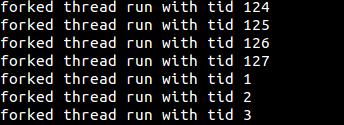
\includegraphics[width=4in]{ex1.png}
\end{figure}

从中可以看出,Yield会触发等待线程队列的队头被执行,所以这里当每个线程被创建前前一个线程就会运行结束,这也是为什么在tid=127后创建的线程又重新从1开始了(0是main线程)。

\textbf{增加一个TS功能,能够显示当前系统中的所有现成的信息和状态}
我觉得这是一个开放性的设计,因为要求中也没有规定TS这个功能具体要实现的什么程度。
从我个人的角度来看,这个TS和调试信息模式有点相似,都是向外输出内部运行情况的,所以我参照调试模式,把TS作为一种模式可在命令行参数中激活。如:

./nachos -q 2 --ts 

就可以在TS模式下执行相应的测试。

我维护了一个全局变量enableTS,默认为false。只有当命令行参数处理过程中识别到--ts后enableTS才会被赋值为true。

这里另一个需要考虑的是TS输出的时机。我在这里选择的是Yield的时候,既每当调用一个线程的Yield,就会自动生成TS信息。
具体的输出方法主要调用了List的Mapcar,这个和函数式语言中的map非常相像,即对List中的所有元素做同一个操作。具体代码如下:
\begin{lstlisting}
void TS_print(int arg) {
    Thread *t = (Thread *) arg;
    printf("Thread %s with threadID %d and userID %d %s\n", 
                t->getName(), 
                t->getTID(),
                t->getUID(),
                t->getStatus());
}

void TS() {
    if(!enableTS) {
        return;
    }
    printf("---------------TS-------------\n");
    printf("Thread %s with threadID %d and userID %d %s\n", 
                currentThread->getName(), 
                currentThread->getTID(),
                currentThread->getUID(),
                currentThread->getStatus());
    if(!scheduler->getReadyList()->IsEmpty()) {
        scheduler->getReadyList()->Mapcar(TS_print);
    }
    printf("------------------------------\n");
}
\end{lstlisting}

以下为TS模式下原来的ThreadTest的输出。
\begin{figure}[h]
 \centering
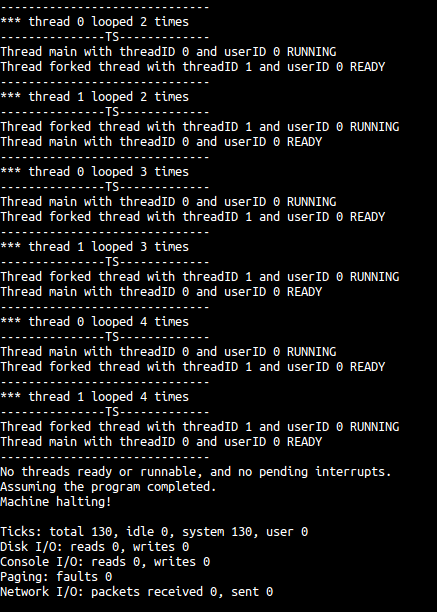
\includegraphics[width=4in]{ex3.png}
\end{figure}

这个test本质上就是两个线程交互地互相运行。所以TS的结果是正确的。
\section{遇到的困难以及解决办法}
我遇到的主要困难有如下:
\subsection*{底层代码}
Nachos中有一些直接与硬件相关的代码。这些代码比较底层,具体实现细节也不是特别重要。但是如果想要真正理解这个系统,底层代码还是需要理解的。对此我还翻出了久违的ICS书,把一些栈的结构都看了一遍,才完全理解了底层的代码,如Thread中的StackAllocate。
\subsection*{中断处理}
中断处理一直是我在操作系统学习上的一个软肋,我一直不能很好的判断什么地方应该关中断。不过我还是按照了常规思路,在TS功能中设置了中断开关,因为TS功能涉及到了长时间的遍历链表和输出,在这个过程中应该尽可能的保证不要被打断。
\subsection*{测试设计与时序分析}
测试的设计也不是很方便,要设计出具有代表性的测试用例,既要对各种可能情形进行考虑,还要深入理解一些时序关系。对此我打开了所有调试信息,并且人工地模拟了代码的执行,分析好了时序。并且设计出了相应的测试用例来测试时序关系。
\section{收获与感想}
这是对一个操作系统的源码扩展的第一次尝试,虽然不是很难,但毕竟初上手,还有一些生疏。

在此过程中,我发现即使工作量已经很小了,但是需要注意的地方很多。需要系统化地考虑整个系统的设计。这次Lab是针对线程机制的,在调研,阅读代码,编写代码,攥写报告的过程中,我对操作系统的线程机制有了更深的理解。

与此同时我还遇到了一些小麻烦,最后找到了解决办法。但我认为可能这些方法还算不上完美,如果真正的要设计好一个系统还是需要尽善尽美的。所以在后面的Lab中我会尽可能地花更多的时间设计出质量更好的代码。

\section{意见与建议}
对于实验来暂无重要的建议。但平时上课发言加分我觉得还是不妥,不如改成发言发奖品但不记名。

\section{参考资料}
\begin{itemize}
\item 《现代操作系统》
\item 《深入理解计算机系统》
\item 《Linux内核设计与实现》
\end{itemize}

\end{document}